\documentclass[12pt]{article}\usepackage[]{graphicx}\usepackage[]{xcolor}
% maxwidth is the original width if it is less than linewidth
% otherwise use linewidth (to make sure the graphics do not exceed the margin)
\makeatletter
\def\maxwidth{ %
  \ifdim\Gin@nat@width>\linewidth
    \linewidth
  \else
    \Gin@nat@width
  \fi
}
\makeatother

\definecolor{fgcolor}{rgb}{0.345, 0.345, 0.345}
\newcommand{\hlnum}[1]{\textcolor[rgb]{0.686,0.059,0.569}{#1}}%
\newcommand{\hlstr}[1]{\textcolor[rgb]{0.192,0.494,0.8}{#1}}%
\newcommand{\hlcom}[1]{\textcolor[rgb]{0.678,0.584,0.686}{\textit{#1}}}%
\newcommand{\hlopt}[1]{\textcolor[rgb]{0,0,0}{#1}}%
\newcommand{\hlstd}[1]{\textcolor[rgb]{0.345,0.345,0.345}{#1}}%
\newcommand{\hlkwa}[1]{\textcolor[rgb]{0.161,0.373,0.58}{\textbf{#1}}}%
\newcommand{\hlkwb}[1]{\textcolor[rgb]{0.69,0.353,0.396}{#1}}%
\newcommand{\hlkwc}[1]{\textcolor[rgb]{0.333,0.667,0.333}{#1}}%
\newcommand{\hlkwd}[1]{\textcolor[rgb]{0.737,0.353,0.396}{\textbf{#1}}}%
\let\hlipl\hlkwb

\usepackage{framed}
\makeatletter
\newenvironment{kframe}{%
 \def\at@end@of@kframe{}%
 \ifinner\ifhmode%
  \def\at@end@of@kframe{\end{minipage}}%
  \begin{minipage}{\columnwidth}%
 \fi\fi%
 \def\FrameCommand##1{\hskip\@totalleftmargin \hskip-\fboxsep
 \colorbox{shadecolor}{##1}\hskip-\fboxsep
     % There is no \\@totalrightmargin, so:
     \hskip-\linewidth \hskip-\@totalleftmargin \hskip\columnwidth}%
 \MakeFramed {\advance\hsize-\width
   \@totalleftmargin\z@ \linewidth\hsize
   \@setminipage}}%
 {\par\unskip\endMakeFramed%
 \at@end@of@kframe}
\makeatother

\definecolor{shadecolor}{rgb}{.97, .97, .97}
\definecolor{messagecolor}{rgb}{0, 0, 0}
\definecolor{warningcolor}{rgb}{1, 0, 1}
\definecolor{errorcolor}{rgb}{1, 0, 0}
\newenvironment{knitrout}{}{} % an empty environment to be redefined in TeX

\usepackage{alltt}

\usepackage{caption}
\usepackage{subcaption}

\usepackage{algpseudocode}
\usepackage{algorithm}

\usepackage{tikz}
\usetikzlibrary{shadows}
\usetikzlibrary{bayesnet} 
\usepackage[margin=1in]{geometry}

\setlength\parindent{0pt}
\IfFileExists{upquote.sty}{\usepackage{upquote}}{}
\begin{document}

\begin{center}
\Large \underline{Metrics to Assess Algorithm Performance}
\end{center}

Mixed graph markings:
\begin{enumerate}
\item[0] Nothing (no edge exists)
\item[1] Undetermined 
\item[2] Arrowhead
\item[3] Tail
\end{enumerate}
Note: The $\ast$ mark used in these rules represents a wildcard that denotes any of the three marks. If this symbol appears in the consequent of a rule, then the remark remains the same as it was in the antecedent.

\begin{knitrout}
\definecolor{shadecolor}{rgb}{0.969, 0.969, 0.969}\color{fgcolor}\begin{kframe}
\begin{alltt}
\hlkwd{library}\hlstd{(LocalFCI)}
\end{alltt}


{\ttfamily\noindent\itshape\color{messagecolor}{\#\# Loading required package: bnlearn}}\begin{alltt}
\hlkwd{data}\hlstd{(}\hlstr{"asiaDAG"}\hlstd{)}
\hlkwd{data}\hlstd{(}\hlstr{"asiadf"}\hlstd{)}
\hlstd{asiadf} \hlkwb{<-} \hlkwd{as.matrix}\hlstd{(asiadf)}
\end{alltt}
\end{kframe}
\end{knitrout}

\section*{Introduction}
For all metrics, we are comparing the adjacency matrix of an estimated graph to a graph regarded as the ``ground truth.'' In our simulations, we regard the subgraph of the CPDAG as the ground truth we will measure our estimates against. The subgraph contains all of the target nodes and the union of their neighborhoods.

\section*{\texttt{allMetrics}}
In this section, we will check the validity of the constituent functions producing the metrics returned by this function. The implementation for all of these may be found in \texttt{metrics.cpp}.
\newpage
\subsection*{Skeleton Estimation Metrics}
\begin{knitrout}
\definecolor{shadecolor}{rgb}{0.969, 0.969, 0.969}\color{fgcolor}\begin{kframe}
\begin{alltt}
\hlstd{true_amat} \hlkwb{<-} \hlkwd{matrix}\hlstd{(}\hlkwd{c}\hlstd{(}\hlnum{0}\hlstd{,}\hlnum{1}\hlstd{,}\hlnum{0}\hlstd{,}\hlnum{0}\hlstd{,}
                      \hlnum{1}\hlstd{,}\hlnum{0}\hlstd{,}\hlnum{1}\hlstd{,}\hlnum{1}\hlstd{,}
                      \hlnum{0}\hlstd{,}\hlnum{0}\hlstd{,}\hlnum{0}\hlstd{,}\hlnum{1}\hlstd{,}
                      \hlnum{0}\hlstd{,}\hlnum{0}\hlstd{,}\hlnum{0}\hlstd{,}\hlnum{0}\hlstd{),}\hlkwc{byrow} \hlstd{=} \hlnum{TRUE}\hlstd{,}\hlkwc{nrow} \hlstd{=} \hlnum{4}\hlstd{)}

\hlstd{perfect_skel} \hlkwb{<-} \hlkwd{matrix}\hlstd{(}\hlkwd{c}\hlstd{(}\hlnum{0}\hlstd{,}\hlnum{1}\hlstd{,}\hlnum{0}\hlstd{,}\hlnum{0}\hlstd{,}
                         \hlnum{0}\hlstd{,}\hlnum{0}\hlstd{,}\hlnum{0}\hlstd{,}\hlnum{1}\hlstd{,}
                         \hlnum{0}\hlstd{,}\hlnum{1}\hlstd{,}\hlnum{0}\hlstd{,}\hlnum{1}\hlstd{,}
                         \hlnum{0}\hlstd{,}\hlnum{0}\hlstd{,}\hlnum{0}\hlstd{,}\hlnum{0}\hlstd{),}\hlkwc{byrow} \hlstd{=} \hlnum{TRUE}\hlstd{,}\hlkwc{nrow} \hlstd{=} \hlnum{4}\hlstd{)}

\hlstd{false_skel} \hlkwb{<-} \hlkwd{matrix}\hlstd{(}\hlkwd{c}\hlstd{(}\hlnum{0}\hlstd{,}\hlnum{0}\hlstd{,}\hlnum{1}\hlstd{,}\hlnum{1}\hlstd{,}
                       \hlnum{0}\hlstd{,}\hlnum{0}\hlstd{,}\hlnum{1}\hlstd{,}\hlnum{1}\hlstd{,}
                       \hlnum{0}\hlstd{,}\hlnum{0}\hlstd{,}\hlnum{0}\hlstd{,}\hlnum{0}\hlstd{,}
                       \hlnum{0}\hlstd{,}\hlnum{0}\hlstd{,}\hlnum{0}\hlstd{,}\hlnum{0}\hlstd{),}\hlkwc{byrow} \hlstd{=} \hlnum{TRUE}\hlstd{,}\hlkwc{nrow} \hlstd{=} \hlnum{4}\hlstd{)}
\end{alltt}
\end{kframe}
\end{knitrout}


\begin{knitrout}
\definecolor{shadecolor}{rgb}{0.969, 0.969, 0.969}\color{fgcolor}\begin{figure}
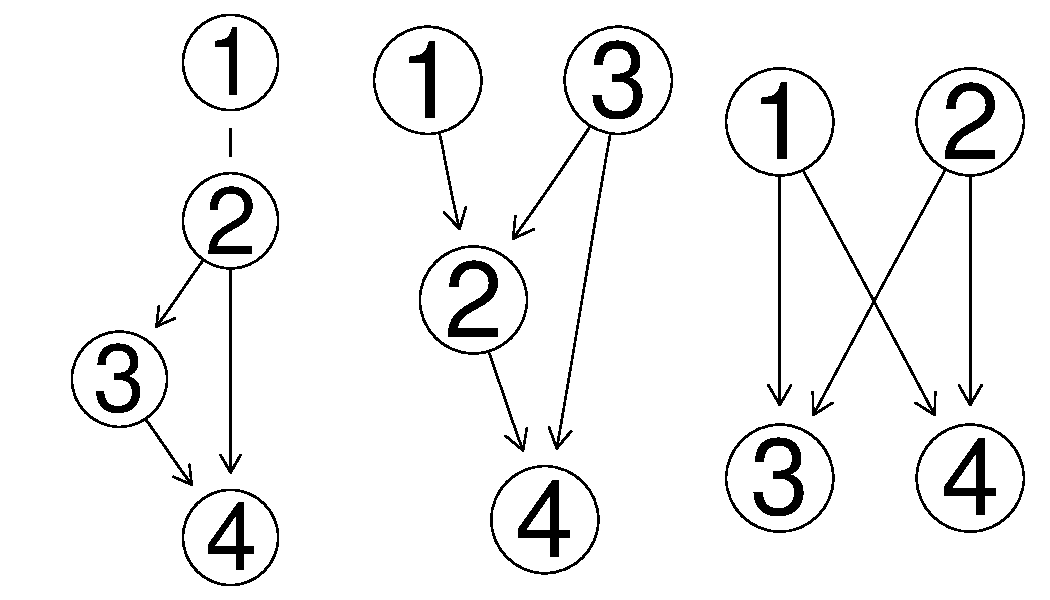
\includegraphics[width=\maxwidth]{figure/unnamed-chunk-3-1} \caption[From left to right, we have the true graph, the graph with the perfect skeleton, and the graph with an incorrect skeleton]{From left to right, we have the true graph, the graph with the perfect skeleton, and the graph with an incorrect skeleton.}\label{fig:unnamed-chunk-3}
\end{figure}

\end{knitrout}

\begin{knitrout}
\definecolor{shadecolor}{rgb}{0.969, 0.969, 0.969}\color{fgcolor}\begin{kframe}
\begin{alltt}
\hlkwd{compareSkeletons}\hlstd{(false_skel,true_amat,}\hlkwc{targets} \hlstd{=} \hlkwd{c}\hlstd{(}\hlnum{1}\hlstd{,}\hlnum{3}\hlstd{))}
\end{alltt}
\begin{verbatim}
## $skel_fp
## [1] 2
## 
## $skel_fn
## [1] 2
## 
## $skel_correct
## [1] 2
\end{verbatim}
\begin{alltt}
\hlkwd{compareSkeletons}\hlstd{(false_skel,true_amat,}\hlkwc{targets} \hlstd{=} \hlnum{3}\hlstd{)}
\end{alltt}
\begin{verbatim}
## $skel_fp
## [1] 0
## 
## $skel_fn
## [1] 1
## 
## $skel_correct
## [1] 2
\end{verbatim}
\begin{alltt}
\hlkwd{compareSkeletons}\hlstd{(perfect_skel,true_amat,}\hlkwc{targets} \hlstd{=} \hlnum{3}\hlstd{)}
\end{alltt}
\begin{verbatim}
## $skel_fp
## [1] 0
## 
## $skel_fn
## [1] 0
## 
## $skel_correct
## [1] 3
\end{verbatim}
\begin{alltt}
\hlkwd{compareSkeletons}\hlstd{(perfect_skel,true_amat,}\hlkwc{targets} \hlstd{=} \hlkwd{c}\hlstd{(}\hlnum{1}\hlstd{,}\hlnum{3}\hlstd{))}
\end{alltt}
\begin{verbatim}
## $skel_fp
## [1] 0
## 
## $skel_fn
## [1] 0
## 
## $skel_correct
## [1] 4
\end{verbatim}
\end{kframe}
\end{knitrout}

Note the differences in the values for each call are due to the differences in the provided target node. The false skeleton correctly has edges $(2,3)$ and $(2,4)$. It is missing edges $(3,4)$ and $(1,2)$. It adds edges $(1,3)$ and $(1,4)$.

In our implementation, we only count edges from nodes that are found in the same target neighborhood in the ground truth. In this way, we won't wrong penalize any remaining edges from our algorithm that link separate neighborhoods.

\subsection*{V-Structure Estimation Metrics}
In this implementation, we again only consider those v-structures found within the same target neighborhood in the ground truth graph, so we will not penalize any v-structures found between target neighborhoods. Also note that this implementation only recognizes notation for a typical graph without additional edge marks.\\

We use the same graphs shown above.

\begin{knitrout}
\definecolor{shadecolor}{rgb}{0.969, 0.969, 0.969}\color{fgcolor}\begin{kframe}
\begin{alltt}
\hlkwd{compareVStructures}\hlstd{(false_skel,true_amat,}\hlkwc{targets} \hlstd{=} \hlkwd{c}\hlstd{(}\hlnum{0}\hlstd{,}\hlnum{3}\hlstd{),}\hlnum{TRUE}\hlstd{)}
\end{alltt}
\begin{verbatim}
## Checking: 1, 2, and 3
## Estimated Graph:
## No unshielded triple
## 
## True Graph:
## No unshielded triple
## $missing
## [1] 0
## 
## $added
## [1] 0
## 
## $correct
## [1] 0
\end{verbatim}
\begin{alltt}
\hlkwd{compareVStructures}\hlstd{(false_skel,true_amat,}\hlkwc{targets} \hlstd{=} \hlnum{3}\hlstd{,}\hlnum{TRUE}\hlstd{)}
\end{alltt}
\begin{verbatim}
## Checking: 1, 2, and 3
## Estimated Graph:
## No unshielded triple
## 
## True Graph:
## No unshielded triple
## $missing
## [1] 0
## 
## $added
## [1] 0
## 
## $correct
## [1] 0
\end{verbatim}
\begin{alltt}
\hlkwd{compareVStructures}\hlstd{(perfect_skel,true_amat,}\hlkwc{targets} \hlstd{=} \hlnum{1}\hlstd{,}\hlnum{TRUE}\hlstd{)}
\end{alltt}
\begin{verbatim}
## Checking: 0, 1, and 2
## Estimated Graph:
## 0 -> 1 <- 2
## True Graph:
## v-structure *not* present in other graph
## True Graph:
## No unshielded triple
## 
## Checking: 0, 1, and 3
## Estimated Graph:
## No unshielded triple
## 
## True Graph:
## No unshielded triple
## 
## Checking: 0, 2, and 3
## Estimated Graph:
## No unshielded triple
## 
## True Graph:
## No unshielded triple
## 
## Checking: 1, 2, and 3
## Estimated Graph:
## No unshielded triple
## 
## True Graph:
## No unshielded triple
## $missing
## [1] 0
## 
## $added
## [1] 1
## 
## $correct
## [1] 0
\end{verbatim}
\begin{alltt}
\hlkwd{compareVStructures}\hlstd{(false_skel,true_amat,}\hlkwc{targets} \hlstd{=} \hlnum{1}\hlstd{,}\hlnum{TRUE}\hlstd{)}
\end{alltt}
\begin{verbatim}
## Checking: 0, 1, and 2
## Estimated Graph:
## 0 -> 2 <- 1
## True Graph:
## v-structure *not* present in other graph
## True Graph:
## No unshielded triple
## 
## Checking: 0, 1, and 3
## Estimated Graph:
## 0 -> 3 <- 1
## True Graph:
## v-structure *not* present in other graph
## True Graph:
## No unshielded triple
## 
## Checking: 0, 2, and 3
## Estimated Graph:
## No unshielded triple
## 
## True Graph:
## No unshielded triple
## 
## Checking: 1, 2, and 3
## Estimated Graph:
## No unshielded triple
## 
## True Graph:
## No unshielded triple
## $missing
## [1] 0
## 
## $added
## [1] 2
## 
## $correct
## [1] 0
\end{verbatim}
\end{kframe}
\end{knitrout}

\subsection*{Parent Recovery Metrics}
One of the primary goals of this algorithm is to properly identify parents of target nodes so that we can estimate the causal effects on downstream nodes.

In our accounting of target parent recovery, we identify true positives, false negatives, and false positives. In addition, we have another category called ``potential'' parents. These nodes could be 
\begin{itemize}
\item An identified parent in the estimated graph where there is an undirected edge in the ground truth
\item An undirected edge in the estimated graph where there is a parental relationship identified in the ground truth
\item Undirected edges in both the estimated graph and the true graph
\end{itemize}

\begin{knitrout}
\definecolor{shadecolor}{rgb}{0.969, 0.969, 0.969}\color{fgcolor}\begin{kframe}
\begin{alltt}
\hlkwd{parentRecoveryAccuracy}\hlstd{(perfect_skel,true_amat,}\hlkwc{targets} \hlstd{=} \hlnum{3}\hlstd{)}
\end{alltt}
\begin{verbatim}
## $missing
## [1] 0
## 
## $added
## [1] 0
## 
## $correct
## [1] 2
## 
## $potential
## [1] 0
\end{verbatim}
\begin{alltt}
\hlkwd{parentRecoveryAccuracy}\hlstd{(false_skel,true_amat,}\hlkwc{targets} \hlstd{=} \hlnum{3}\hlstd{)}
\end{alltt}
\begin{verbatim}
## $missing
## [1] 1
## 
## $added
## [1] 1
## 
## $correct
## [1] 1
## 
## $potential
## [1] 0
\end{verbatim}
\begin{alltt}
\hlkwd{parentRecoveryAccuracy}\hlstd{(false_skel,true_amat,}\hlkwc{targets} \hlstd{=} \hlkwd{c}\hlstd{(}\hlnum{0}\hlstd{,}\hlnum{3}\hlstd{))}
\end{alltt}
\begin{verbatim}
## $missing
## [1] 1
## 
## $added
## [1] 1
## 
## $correct
## [1] 1
## 
## $potential
## [1] 0
\end{verbatim}
\end{kframe}
\end{knitrout}

Next, we add an undirected edge in the graph with the false skeleton and observe the changes this makes in the reported metrics on parent recovery.
\begin{knitrout}
\definecolor{shadecolor}{rgb}{0.969, 0.969, 0.969}\color{fgcolor}\begin{kframe}
\begin{alltt}
\hlcom{# Adding a potential}
\hlstd{false_skel[}\hlnum{3}\hlstd{,}\hlnum{4}\hlstd{]} \hlkwb{<-} \hlnum{1}
\hlstd{false_skel[}\hlnum{4}\hlstd{,}\hlnum{3}\hlstd{]} \hlkwb{<-} \hlnum{1}
\hlkwd{parentRecoveryAccuracy}\hlstd{(false_skel,true_amat,}\hlkwc{targets} \hlstd{=} \hlnum{3}\hlstd{)}
\end{alltt}
\begin{verbatim}
## $missing
## [1] 1
## 
## $added
## [1] 1
## 
## $correct
## [1] 1
## 
## $potential
## [1] 1
\end{verbatim}
\begin{alltt}
\hlcom{# Using 1-index numbering: }
\hlcom{# Missing 3 -> 4, correctly has 2->3 and 2->4, has 3-4 as undirected edge, }
\hlcom{# added 1->4 and 1->3}
\hlkwd{parentRecoveryAccuracy}\hlstd{(false_skel,true_amat,}\hlkwc{targets} \hlstd{=} \hlkwd{c}\hlstd{(}\hlnum{2}\hlstd{,}\hlnum{3}\hlstd{))}
\end{alltt}
\begin{verbatim}
## $missing
## [1] 1
## 
## $added
## [1] 2
## 
## $correct
## [1] 2
## 
## $potential
## [1] 1
\end{verbatim}
\begin{alltt}
\hlkwd{parentRecoveryAccuracy}\hlstd{(false_skel,true_amat,}\hlkwc{targets} \hlstd{=} \hlkwd{c}\hlstd{(}\hlnum{1}\hlstd{,}\hlnum{2}\hlstd{,}\hlnum{3}\hlstd{))}
\end{alltt}
\begin{verbatim}
## $missing
## [1] 1
## 
## $added
## [1] 2
## 
## $correct
## [1] 2
## 
## $potential
## [1] 1
\end{verbatim}
\end{kframe}
\end{knitrout}

Change the edge to a bi-directed edge using the values from mixed graphs to observe the changes once again.
\begin{knitrout}
\definecolor{shadecolor}{rgb}{0.969, 0.969, 0.969}\color{fgcolor}\begin{kframe}
\begin{alltt}
\hlstd{false_skel[}\hlnum{3}\hlstd{,}\hlnum{4}\hlstd{]} \hlkwb{<-} \hlnum{2}
\hlstd{false_skel[}\hlnum{4}\hlstd{,}\hlnum{3}\hlstd{]} \hlkwb{<-} \hlnum{2}
\hlkwd{parentRecoveryAccuracy}\hlstd{(false_skel,true_amat,}\hlkwc{targets} \hlstd{=} \hlnum{3}\hlstd{)}
\end{alltt}
\begin{verbatim}
## $missing
## [1] 1
## 
## $added
## [1] 1
## 
## $correct
## [1] 1
## 
## $potential
## [1] 0
\end{verbatim}
\end{kframe}
\end{knitrout}

\subsection*{Inter-Neighborhood Edge Metrics}

One of the advantages of using the local FCI algorithm is that we are able to retain and orient some of the edges between neighborhoods. These metrics intend to demonstrate the value of this algorithm in identifying these relationships.

\begin{algorithm}[H]
\footnotesize
\caption{Inter-Neighborhood Edge Metrics}
\begin{algorithmic}[1]
\State \textbf{Input:} Estimated graph adj. matrix \texttt{est}, Ground truth graph adj. matrix \texttt{ref}
\State Find pairs of nodes $(i,j)$ that are in different target neighborhoods
\If {Nodes $i$ and $j$ are not connected in the estimated graph}
\If {Node $j$ (or $i$) is an ancestor of node $i$ ($j$), and the path from $j$ to $i$ ($i$ to $j$) is unmediated by another considered node}
\State Increment the number of missing ancestral relationships
\EndIf
\Else
\If {The edge is oriented with a proper unmediated ancestral relationship}
\State Increment the number of true ancestors
\ElsIf {The edge is undirected or bidirected}
\State Increment the number of those missing orientation
\ElsIf {The edge reverses the ancestral relationship and the path is unmediated}
\State Increment the number with reversed orientations
\ElsIf {There is a directed edge present without an ancestral relationship}
\State Increment the number of false positive arrowheads
\Else 
\State Increment the number of false positive connections
\EndIf
\EndIf
\end{algorithmic}
\end{algorithm}

\subsection*{Overall F1 Score}
\begin{itemize}
\item A true positive (TP) is when the orientation exactly matches in both graphs
\item A true negative is when there is no edge in both graphs
\item A false positive is when there is an edge in the estimated graph but no edge in the true graph
\item A false negative is whenever there is an edge in the true graph which does not exactly match the edge in the estimated graph
\end{itemize}

$$ F_1 = \frac{2\times TP}{2\times TP + FP + FN} $$

\end{document}

